% 第 2 章 Defining Clocks
\bichapter{定义时钟}{Defining Clocks}
\label{chap:clocks}

时序分析的关键一步是准确指定时钟以及时钟效应，例如 latency 与 uncertainty。指定、报告与分析时钟见以下主题：
\begin{itemize}
  \item 创建真实时钟
  \item 创建虚拟时钟
  \item 创建生成时钟
  \item 时钟网络效应
  \item 指定时钟源端延迟
  \item 指定理想网络延迟
  \item 指定时钟不确定性
  \item 指定理想时钟转换时间
  \item 为理想时钟启用 clock-to-data 分析
  \item 时钟的单边性（unateness）
  \item 传播指定的时钟极性
  \item 创建脉冲时钟
  \item 设置并报告最小脉冲宽度约束
  \item 定义时钟组之间的关系
  \item 报告时钟相关信息
  \item 删除时钟
\end{itemize}

\section{创建真实时钟}
\subsection*{Creating Real Clocks}

真实时钟（real clock）是物理上存在、定义在 block 的 pin 或 port 对象上的时钟。用 \cmd{create\_clock} 创建真实时钟，并指定：
\begin{itemize}
  \item 用 \opt{-period} 给出时钟周期。
  \item 创建时钟所用的源对象（pin 或 port）。若不指定源对象，工具会创建一个虚拟时钟。
\end{itemize}

还可以指定：
\begin{itemize}
  \item 用 \opt{-waveform} 给出波形。若不指定，默认占空比为 50\%，上升沿在时刻 0，下降沿在半周期处。
  \item 用 \opt{-name} 给出时钟名。若不显式命名，时钟名取自源对象。
  \item 用 \opt{-add} 在同一源对象上再定义时钟。此时必须用 \opt{-name} 为附加时钟命名。
\end{itemize}

下列命令在端口 \cmd{CLK} 上创建一个时钟，并在同一端口上再创建一个名为 \cmd{CLK\_1} 的时钟，其上升沿在 1.0、下降沿在 2.0：
\begin{lstlisting}
icc2_shell> create_clock -period 5.0 [get_ports CLK]
icc2_shell> create_clock -period 4.0 -waveform {1.0 2.0} \
    -name CLK_1 -add [get_ports CLK]
\end{lstlisting}

\section{创建虚拟时钟}
\subsection*{Creating Virtual Clocks}

虚拟时钟（virtual clock）在物理上不存在，但可以用来约束 block。用 \cmd{create\_clock} 创建虚拟时钟，并指定：
\begin{itemize}
  \item 用 \opt{-period} 给出周期。
  \item 用 \opt{-name} 给出时钟名。
\end{itemize}

还可以用 \opt{-waveform} 指定波形。若不指定，默认占空比为 50\%，上升沿在时刻 0，下降沿在半周期处。

下列命令创建名为 \cmd{CLK\_VIR}、使用默认波形的时钟：
\begin{lstlisting}
icc2_shell> create_clock -period 5.0 -name CLK_VIR
\end{lstlisting}

\section{创建生成时钟}
\subsection*{Creating Generated Clocks}

基于另一时钟产生的时钟称为生成时钟（generated clock）。下图给出二分频生成时钟的时钟产生逻辑，以及原始（master）时钟与生成时钟的理想波形。

\begin{figure}[htbp]
  \centering
  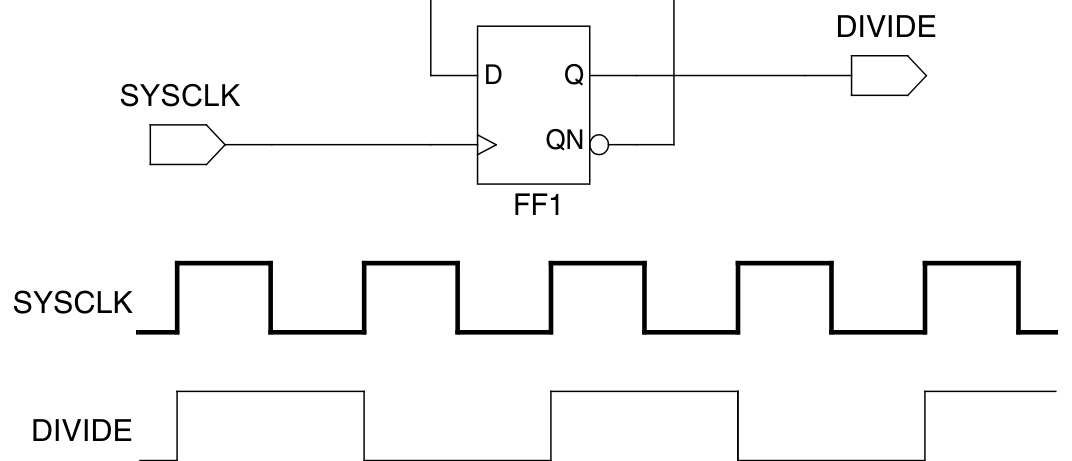
\includegraphics[width=0.85\textwidth]{fig-2-1.png}
  \caption{二分频时钟发生器}
  \label{fig:div2}
\end{figure}

工具不会从逻辑推导生成时钟的行为。必须用 \cmd{create\_generated\_clock}，按 master 时钟来说明生成时钟的行为，并指定：
\begin{itemize}
  \item 创建生成时钟所用的源对象（port、pin 或 net）。
  \item 用 \opt{-source} 指定 master 时钟的源。
  \item 用下列三种方法之一说明频率或波形如何从 master 时钟导出：
  \begin{itemize}
    \item 用 \opt{-divide\_by} 并给出分频因子，由 master 时钟频率除以该因子得到生成时钟频率。
    \item 用 \opt{-multiply\_by} 并给出倍频因子，由 master 时钟频率乘以该因子得到生成时钟频率。
    \item 用 \opt{-edges} 并列出要使用的 master 时钟边沿，按指定边沿导出波形。
  \end{itemize}
\end{itemize}

还可以：
\begin{itemize}
  \item 用 \opt{-name} 为生成时钟命名。若不命名，工具使用源对象列表中第一个对象的名称。
  \item 用 \opt{-add} 在同一生成时钟源对象上添加多个生成时钟。此时必须用 \opt{-master\_clock} 为附加生成时钟指定 master 时钟。
  \item 用 \opt{-combinational}，在计算生成时钟的 source latency 时只考虑生成时钟源与 master 时钟源之间的组合路径。默认情况下，时序分析同时考虑这两点之间的组合路径与时序路径。
  \item 对用 \opt{-divide\_by} 或 \opt{-multiply\_by} 创建的生成时钟，用 \opt{-invert} 反相波形。
  \item 对用 \opt{-multiply\_by} 创建的生成时钟，用 \opt{-duty\_cycle} 改变占空比。
  \item 对用 \opt{-edges} 从 master 时钟指定边沿导出的生成时钟，用 \opt{-edge\_shift} 延迟或平移所选边沿。
\end{itemize}

\subsection{生成时钟示例}
\subsubsection*{Generated Clock Examples}

下例创建两个生成时钟 \cmd{DIV2A} 与 \cmd{DIV2A\_INV}，频率为 master 时钟 \cmd{CLKA} 的一半。此外，\cmd{DIV2A\_INV} 的波形相对 master 时钟反相。
\begin{lstlisting}
icc2_shell> create_generated_clock -name DIV2A \
    -source [get_ports CLKA] -divide_by 2 \
    [get_pins U15/Q]
icc2_shell> create_generated_clock -name DIV2A_INV \
    -source [get_ports CLKA] -divide_by 2 -invert \
    [get_pins U15/QN]
\end{lstlisting}

下图给出该例中 master 时钟与生成时钟的波形。

\begin{figure}[htbp]
  \centering
  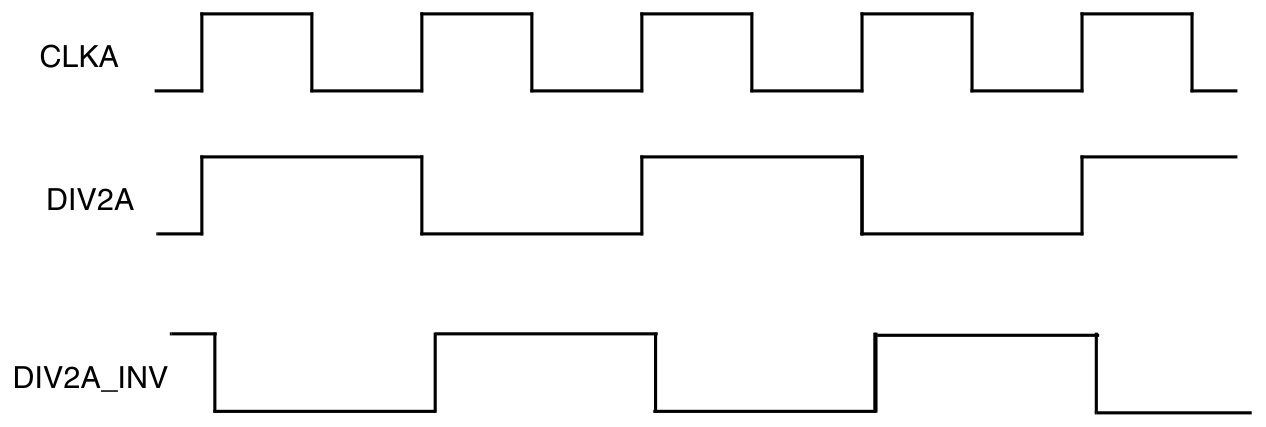
\includegraphics[width=0.9\textwidth]{fig-2-2.png}
  \caption{master 时钟与二分频生成时钟的波形}
  \label{fig:div2-wf}
\end{figure}

下例创建生成时钟 \cmd{MULT2B}，频率为 master 时钟 \cmd{CLKB} 的两倍，有效占空比为 75\%。
\begin{lstlisting}
icc2_shell> create_generated_clock -name MULT2B -duty_cycle 75 \
    -source [get_ports CLKB] -multiply_by 2 \
    [get_pins U29/GC]
\end{lstlisting}

\begin{figure}[htbp]
  \centering
  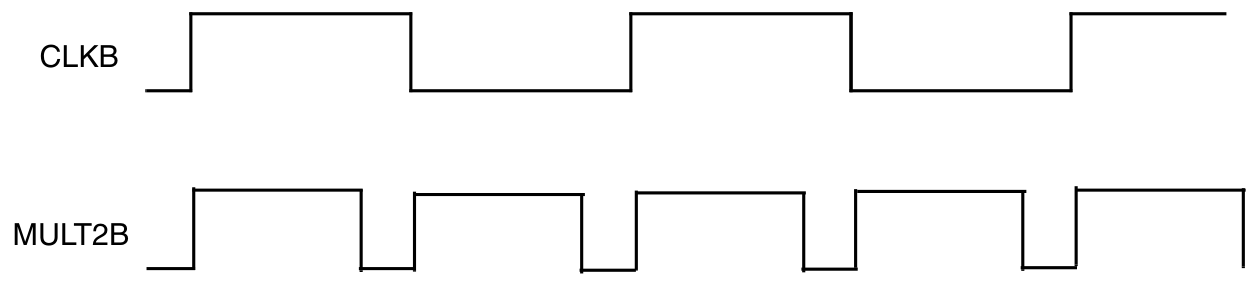
\includegraphics[width=0.9\textwidth]{fig-2-3.png}
  \caption{master 时钟与二倍频生成时钟的波形}
  \label{fig:mult2-wf}
\end{figure}

下例创建 master 时钟 \cmd{CLKC}，以及波形基于 master 时钟第 3、第 5 与第 9 个边沿、且每个边沿平移 2.2 个时间单位的生成时钟 \cmd{DIV3C}。
\begin{lstlisting}
icc2_shell> create_clock -period 2.2 -name CLKC [get_ports CLKC]
icc2_shell> create_generated_clock -name DIV3C \
    -edges {3 5 9} -edge_shift {2.2 2.2 2.2} \
    -source [get_ports SYSCLK] [get_pins U41/QN]
\end{lstlisting}

\cmd{report\_clocks} 按如下方式报告这些时钟：
\begin{lstlisting}
    p - propagated_clock
    G - Generated clock
Clock          Period   Waveform        Attrs     Sources
-------------------------------------------------------------
CLKC           2.20     {0 1.1}                   {CLKC}
DIV3C          6.60     {4.4 6.6}       G         {U41/Q}
Generated     Master       Generated    Waveform
Clock         Source       Source       Modification
-------------------------------------------------------------
DIV3C         MYCLK        U41/Q        edges( 3 5 9 )
                                        shifts( 2.2 2.2 2.2 )
\end{lstlisting}

\begin{figure}[htbp]
  \centering
  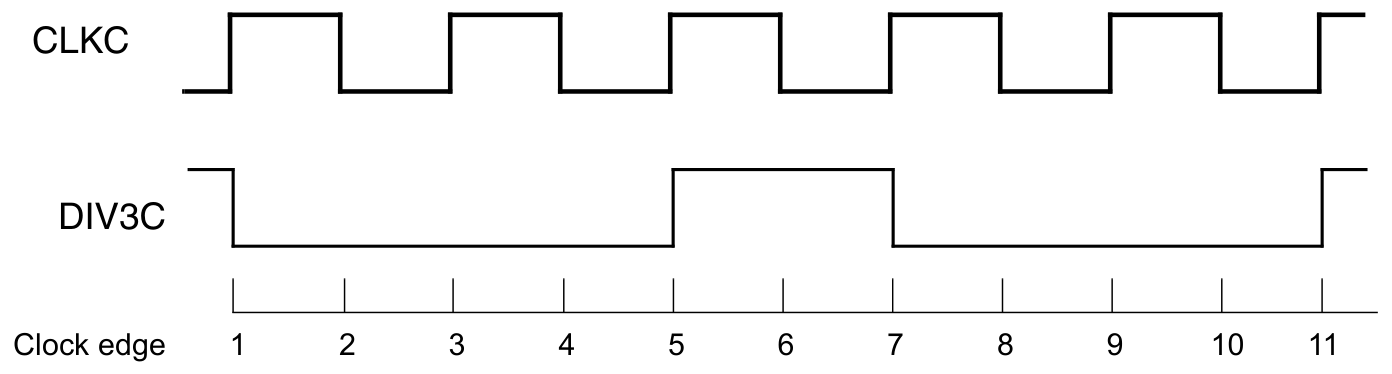
\includegraphics[width=0.92\textwidth]{fig-2-4.png}
  \caption{master 时钟与边沿平移后的三分频生成时钟波形}
  \label{fig:div3-wf}
\end{figure}

下例创建生成时钟 \cmd{CLKD\_INV}，并指定计算该生成时钟的 source latency 时，只使用生成时钟源与 master 时钟源之间的组合路径：
\begin{lstlisting}
icc2_shell> create_generated_clock -name CLKD_INV -divide_by 1 \
    -combinational -source [get_ports CLKD] [get_pins U52/Y]
\end{lstlisting}

下图给出该例中生成时钟源与 master 时钟源之间的全部可用路径。

\begin{figure}[htbp]
  \centering
  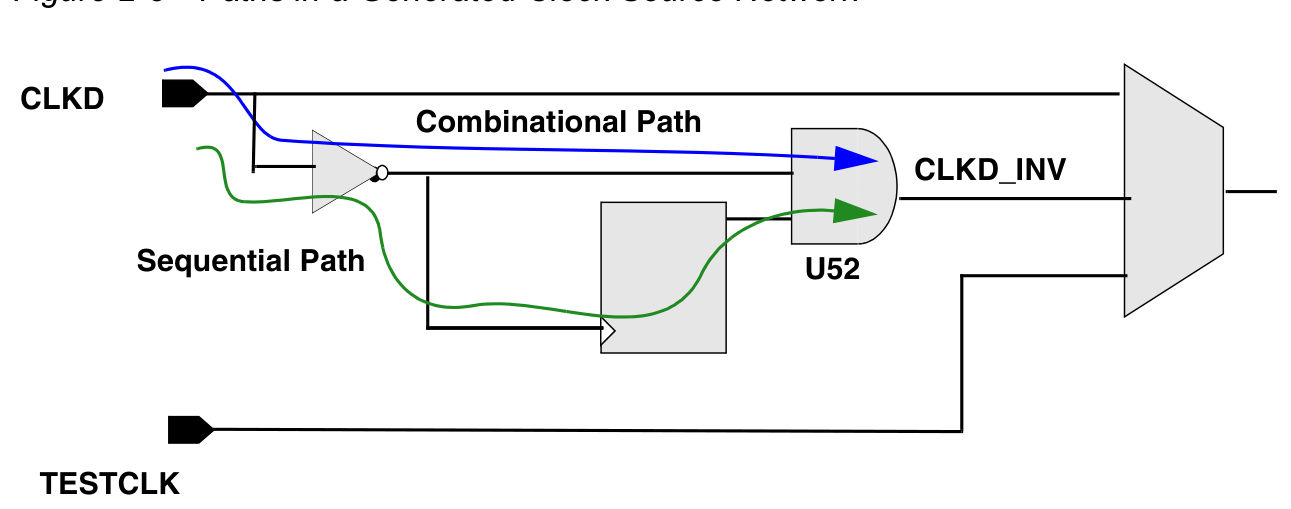
\includegraphics[width=0.85\textwidth]{fig-2-5.png}
  \caption{生成时钟源网络中的路径}
  \label{fig:gen-src-paths}
\end{figure}

\section{时钟网络效应}
\subsection*{Clock Network Effects}

时钟网络具有下列特性。

\begin{itemize}
  \item \textbf{Latency}\\
        时钟信号从原始时钟源传播到设计中时序单元所经历的时间。Latency 由两部分组成：
  \begin{itemize}
    \item Source latency：从时钟源到设计中时钟定义引脚的延迟。
    \item Network latency：从时钟定义点到寄存器时钟引脚的延迟。
  \end{itemize}
        表示 network latency 有两种方法：
  \begin{itemize}
    \item 估计并显式指定每个时钟的 latency。这称为理想网络延迟（ideal network latency），对应时钟称为理想时钟。理想时钟通常用在时钟树综合之前。
    \item 让工具沿时钟网络传播延迟来计算 latency。这称为传播网络延迟（propagated network latency），对应时钟称为传播时钟。传播时钟应只在时钟树综合之后使用。
  \end{itemize}
  \item \textbf{Uncertainty}\\
        同一时钟或不同时钟在寄存器时钟引脚上到达时间的最大变化。时钟不确定性有两个分量：
  \begin{itemize}
    \item 时钟抖动（jitter）：相对理想波形，源时钟相继边沿在产生时刻上的变化。
    \item 时钟偏斜（skew）：从 block 的时钟源到不同寄存器时钟引脚的传播延迟不同，所造成的到达时间差。这只适用于时钟树综合之前。时钟树综合之后，skew 已由传播时钟网络延迟计入。
  \end{itemize}
  \item \textbf{Transition time}\\
        信号从逻辑低变到逻辑高（上升时间）或从逻辑高变到逻辑低（下降时间）所需的时间。
\end{itemize}

下图给出时钟网络的时序效应。

\begin{figure}[htbp]
  \centering
  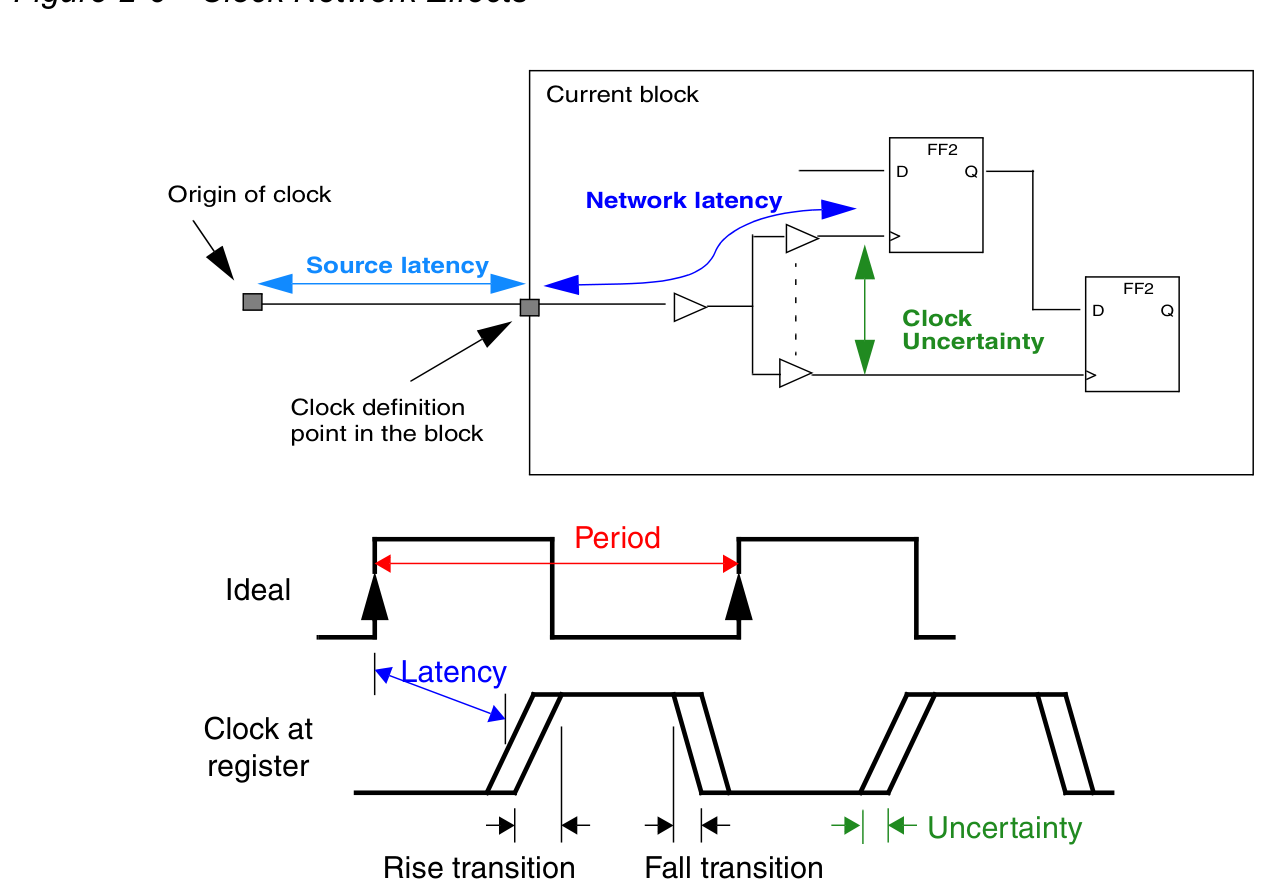
\includegraphics[width=0.88\textwidth]{fig-2-6.png}
  \caption{时钟网络效应}
  \label{fig:clk-net-effects}
\end{figure}

\section{指定时钟源端延迟}
\subsection*{Specifying Clock Source Latency}

对理想时钟与传播时钟都可用 \cmd{set\_clock\_latency -source} 设置 source latency，并指定：
\begin{itemize}
  \item 延迟值。
  \item 受影响的对象列表，可以包含一个或多个时钟、端口或引脚。若对象是 pin 或 port，必须用 \opt{-clock} 指定与该理想网络延迟关联的时钟。
\end{itemize}

还可以指定：
\begin{itemize}
  \item 用 \opt{-early} 与 \opt{-late} 给出 source latency 的 early / late 变化。工具对约束时钟所钟控的每个起点与终点，采用最严的 source latency（early 或 late）。setup 检查对每个起点用 late、对每个终点用 early；hold 检查对每个起点用 early、对每个终点用 late，如下图所示。
\end{itemize}

\begin{figure}[htbp]
  \centering
  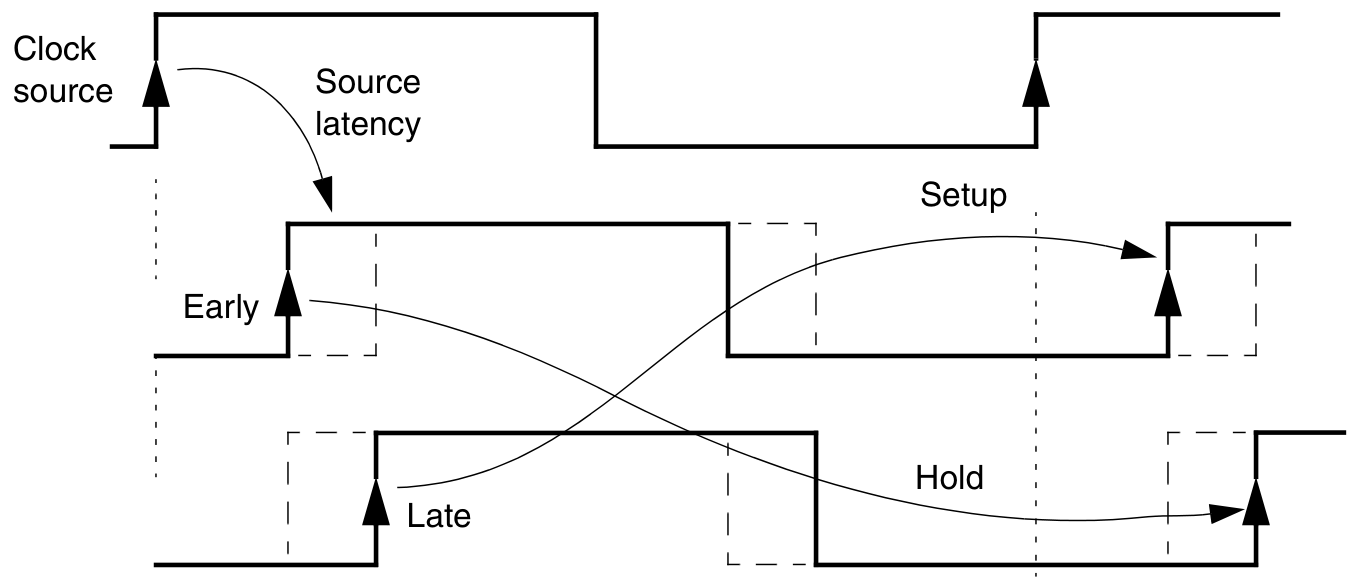
\includegraphics[width=0.85\textwidth]{fig-2-7.png}
  \caption{early 与 late 源端延迟波形}
  \label{fig:early-late-lat}
\end{figure}

\begin{itemize}
  \item 用 \opt{-dynamic} 给出 source latency 的动态变化分量，即相继时钟周期之间不同的那一部分。
\end{itemize}

对多 scenario 设计，source latency 默认只作用于当前 scenario。还可以：
\begin{itemize}
  \item 用 \opt{-modes} 指定某个 mode 的全部 scenario。
  \item 用 \opt{-corners} 指定指定 corner 与当前 mode 的全部 scenario。
  \item 同时用 \opt{-modes} 与 \opt{-corners} 指定指定 mode 与 corner 的全部 scenario。
  \item 用 \opt{-scenarios} 指定具体 scenario。使用该选项时不能再用 \opt{-modes} 或 \opt{-corners}。
\end{itemize}

下列命令把时钟 \cmd{CLK1} 的 source latency 指定为外部时钟网络延迟在 1.5 到 2.5 之间变化，动态分量为 0.5：
\begin{lstlisting}
icc2_shell> set_clock_latency 1.5 -source -early -dynamic 0.5 \
    [get_clocks CLK1]
icc2_shell> set_clock_latency 2.5 -source -late -dynamic 0.5 \
    [get_clocks CLK1]
\end{lstlisting}

用 \cmd{remove\_clock\_latency} 去掉由 \cmd{set\_clock\_latency} 指定的 source latency。

\section{指定理想网络延迟}
\subsection*{Specifying Ideal Network Latency}

用 \cmd{set\_ideal\_network} 把时钟指定为理想时钟。在完成时钟树综合之前，把所有时钟都指定为理想时钟。

用 \cmd{set\_clock\_latency} 指定理想网络延迟，并给出：
\begin{itemize}
  \item 延迟值。
  \item 受影响的对象列表，可以包含一个或多个时钟、端口或引脚。若对象是 pin 或 port，必须用 \opt{-clock} 指定关联时钟。
\end{itemize}

若在时钟网络的某个 pin 或 port 上指定了理想 latency，同时又在对应时钟对象上指定了 latency，则 pin 或 port 上的值作用于其扇出中的全部寄存器时钟引脚，并覆盖加在时钟对象上的 latency。

还可以把理想网络延迟限制为：
\begin{itemize}
  \item 只用 \opt{-rise} 或 \opt{-fall} 作用于上升沿或下降沿。否则同时作用于两个沿。
  \item 只用 \opt{-min} 或 \opt{-max} 作用于最小或最大工作条件。否则作用于全部工作条件。
\end{itemize}

对多 scenario 设计，理想时钟 latency 默认只作用于当前 scenario。指定范围的方式与 source latency 相同：\opt{-modes}、\opt{-corners}、两者同时，或 \opt{-scenarios}。使用 \opt{-scenarios} 时不能再用 \opt{-modes} 或 \opt{-corners}。

下例为当前设计中名为 \cmd{CLK1} 的时钟把期望的上升 latency 设为 1.2、下降 latency 设为 0.9：
\begin{lstlisting}
icc2_shell> set_clock_latency -rise 1.2 [get_clocks CLK1]
icc2_shell> set_clock_latency -fall 0.9 [get_clocks CLK1]
\end{lstlisting}

用 \cmd{remove\_clock\_latency} 去掉由 \cmd{set\_clock\_latency} 指定的理想网络延迟。

\section{指定时钟不确定性}
\subsection*{Specifying Clock Uncertainty}

用 \cmd{set\_clock\_uncertainty} 指定时钟不确定性，给出不确定性数值以及下列之一：
\begin{itemize}
  \item 简单不确定性或抖动：同一时钟相继边沿之间的不确定性。对象列表由时钟、端口或引脚组成。简单不确定性作用于所指定时钟、端口或引脚扇出中的全部寄存器时钟引脚。
  \item 两个时钟之间的时钟间不确定性（interclock uncertainty），用下列方法之一：
  \begin{itemize}
    \item 用 \opt{-from}、\opt{-rise\_from} 或 \opt{-fall\_from} 指定源时钟。
    \item 用 \opt{-to}、\opt{-rise\_to} 或 \opt{-fall\_to} 指定目的时钟。
  \end{itemize}
        指定两个时钟之间的 interclock uncertainty 时，若既有从第一个时钟到第二个时钟的路径，也有反方向路径，即使数值相同，也必须为两个方向都指定不确定性。
\end{itemize}

\begin{figure}[htbp]
  \centering
  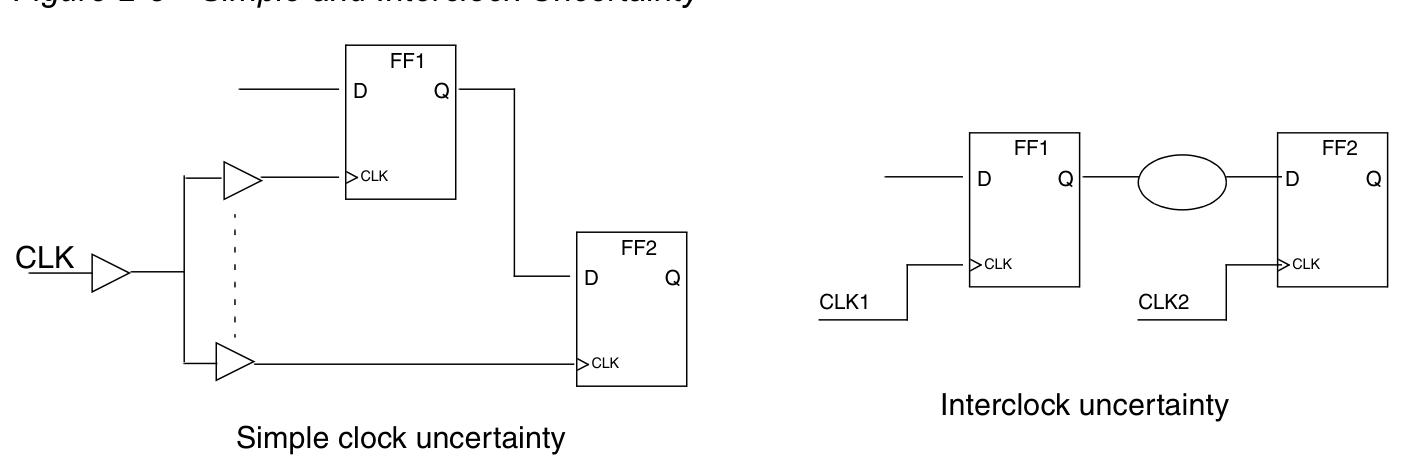
\includegraphics[width=0.92\textwidth]{fig-2-8.png}
  \caption{简单不确定性与时钟间不确定性}
  \label{fig:uncertainty}
\end{figure}

还可以：
\begin{itemize}
  \item 用 \opt{-setup} 指定 setup 检查的简单或时钟间不确定性。
  \item 用 \opt{-hold} 指定 hold 检查的不确定性。
\end{itemize}

对多 scenario 设计，时钟不确定性默认只作用于当前 scenario。指定范围同样使用 \opt{-modes}、\opt{-corners}、两者同时，或 \opt{-scenarios}。使用 \opt{-scenarios} 时不能再用 \opt{-modes} 或 \opt{-corners}。

例如，对由时钟 \cmd{CLK1} 钟控的终点，把简单 setup 不确定性设为 0.21、hold 不确定性设为 0.33：
\begin{lstlisting}
icc2_shell> set_clock_uncertainty -setup 0.21 [get_clocks CLK1]
icc2_shell> set_clock_uncertainty -hold 0.33 [get_clocks CLK1]
\end{lstlisting}

把时钟 \cmd{CLKA} 与 \cmd{CLKB} 之间的 interclock uncertainty 设为 2（setup 与 hold 都设置）：
\begin{lstlisting}
icc2_shell> set_clock_uncertainty 2 -from [get_clocks CLKA] \
    -to [get_clocks CLKB]
icc2_shell> set_clock_uncertainty 2 -from [get_clocks CLKB] \
    -to [get_clocks CLKA]
\end{lstlisting}

用 \cmd{remove\_clock\_uncertainty} 去掉时钟不确定性设置。

\section{指定理想时钟转换时间}
\subsection*{Specifying Ideal Clock Transition}

理想时钟的默认转换时间为零。要用 \cmd{set\_clock\_transition} 为理想时钟指定非零转换时间，并给出：
\begin{itemize}
  \item 理想转换时间值。
  \item 它作用的时钟列表。
\end{itemize}

还可以限定转换时间只作用于：
\begin{itemize}
  \item 用 \opt{-rise} 或 \opt{-fall} 指定的上升沿或下降沿。
  \item 用 \opt{-min} 或 \opt{-max} 指定的最小或最大条件。
\end{itemize}

对多 scenario 设计，理想时钟转换时间默认只作用于当前 scenario。范围选项与前面相同：\opt{-modes}、\opt{-corners}、两者同时，或 \opt{-scenarios}。

工具把所指定的转换时间用于这些时钟传递扇出中的全部寄存器时钟引脚。

例如，在当前 scenario 中，把时钟 \cmd{CLK1} 全部寄存器时钟引脚上的转换时间指定为 0.64：
\begin{lstlisting}
icc2_shell> set_clock_transition 0.64 [get_clocks CLK1]
\end{lstlisting}

用 \cmd{remove\_clock\_transition} 去掉该命令指定的理想转换时间。

\section{为理想时钟启用 clock-to-data 分析}
\subsection*{Enabling Clock-to-Data Analysis for Ideal Clocks}

若时钟到达某个不是时钟引脚（时序引脚）的单元引脚，如下图所示，工具把它识别为 clock-to-data 引脚，并把引脚属性 \cmd{pin\_is\_clock\_to\_data} 设为 \cmd{true}。

\begin{figure}[htbp]
  \centering
  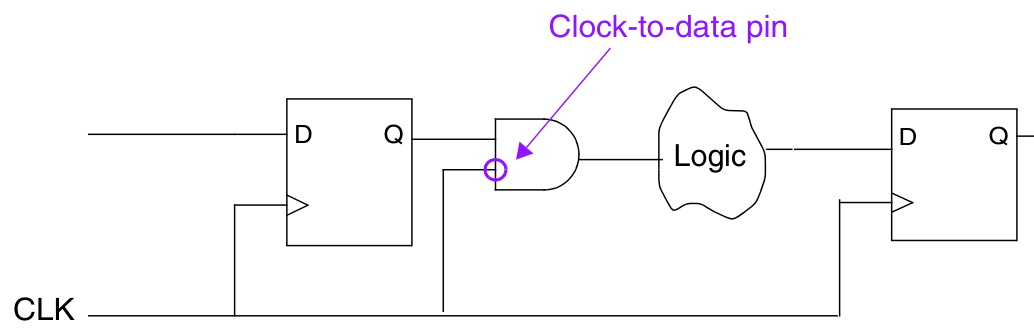
\includegraphics[width=0.72\textwidth]{fig-2-9.png}
  \caption{clock-to-data 引脚}
  \label{fig:c2d}
\end{figure}

可用下列命令找出 block 中的 clock-to-data 引脚：
\begin{lstlisting}
icc2_shell> get_pins -filter "pin_is_clock_to_data==true"
\end{lstlisting}

若传播时钟到达 clock-to-data 引脚，工具把传播时钟到达时间用作该引脚的数据到达时间，把传播时钟转换时间用作数据转换时间。

理想时钟到达 clock-to-data 引脚时，默认不把理想时钟 latency 用作数据到达时间，也不把理想时钟转换时间用作数据转换时间。要把理想时钟的 latency 与转换时间用到该引脚上，把应用选项 \appopt{time.enable\_clock\_to\_data\_analysis} 设为 \cmd{true}。

\section{时钟的单边性}
\subsection*{Unateness of Clocks}

时钟信号分为：
\begin{itemize}
  \item \textbf{Positive unate}：时钟源的上升沿只能在寄存器时钟引脚上引起上升沿，下降沿只能引起下降沿。
  \item \textbf{Negative unate}：时钟源的上升沿只能在寄存器时钟引脚上引起下降沿，下降沿只能引起上升沿。也就是说，时钟信号被反相。
  \item \textbf{Non-unate}：时钟路径中存在 non-unate 时序弧，时钟极性不明确。例如经过 XOR 门的时钟不是 unate 的。极性是正还是负，取决于 XOR 另一输入的状态。
\end{itemize}

下图给出产生 unate 与 non-unate 时钟信号的时钟逻辑示例。

\begin{figure}[htbp]
  \centering
  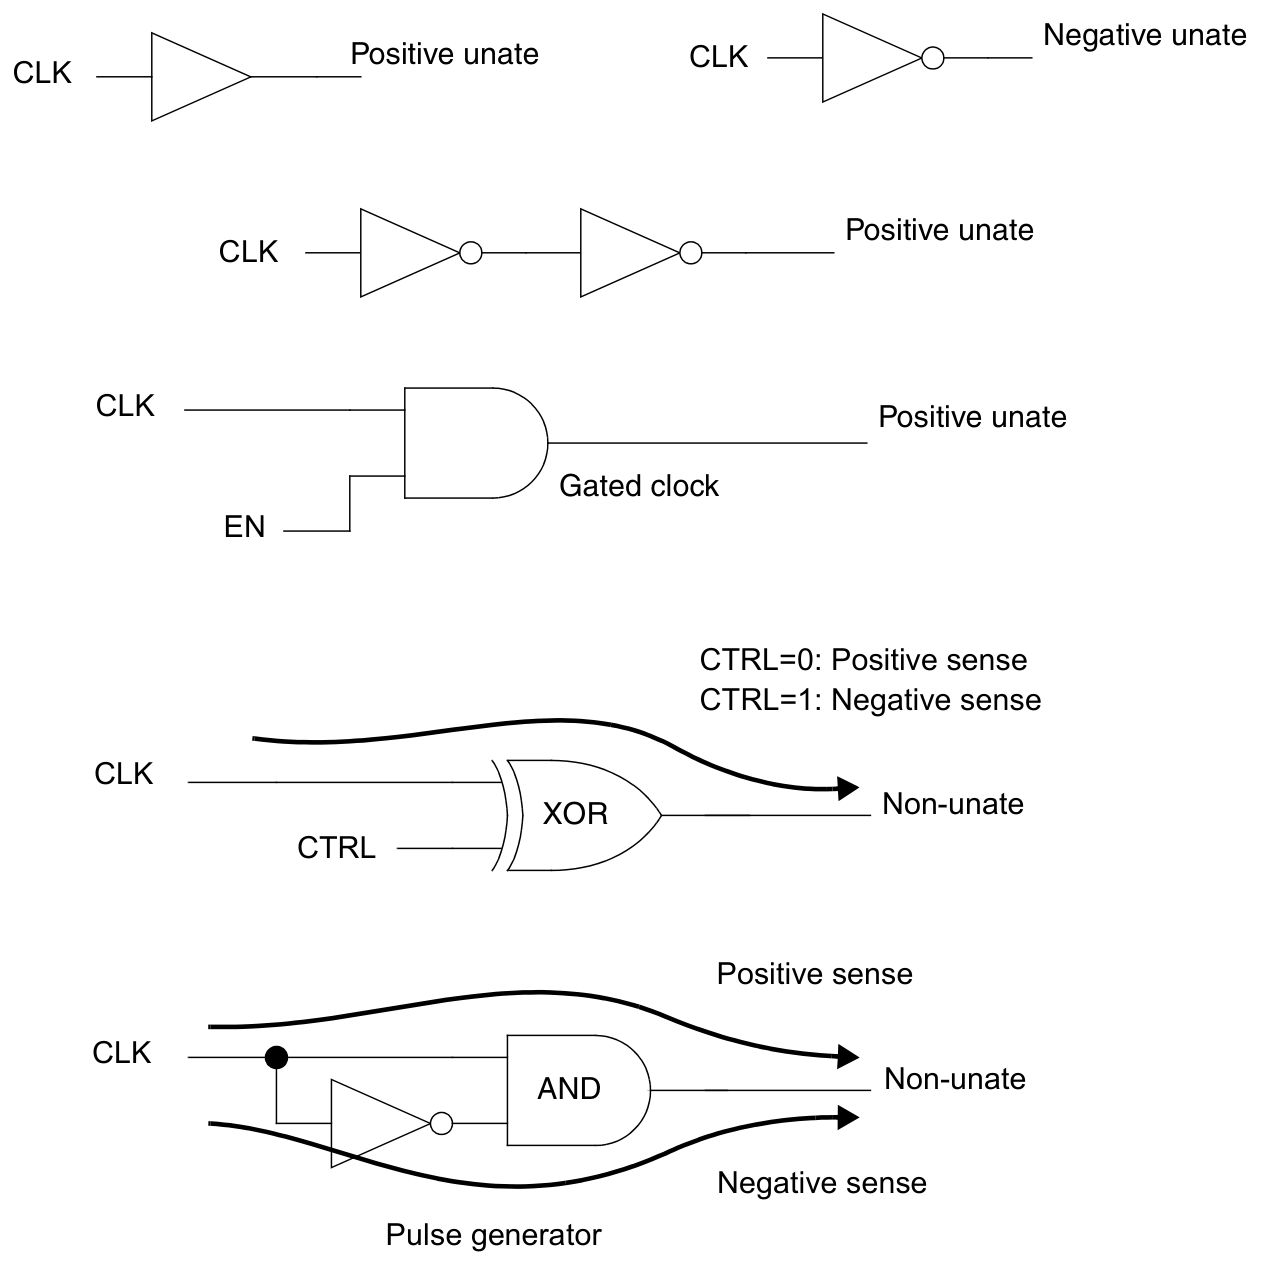
\includegraphics[width=0.82\textwidth]{fig-2-10.png}
  \caption{unate 与 non-unate 时钟信号}
  \label{fig:unate}
\end{figure}

\section{传播指定的时钟极性}
\subsection*{Propagating a Specific Clock Sense}

若时钟网络只含产生 positive unate 或 negative unate 时钟信号的逻辑，工具可以推导到达每个寄存器时钟引脚的时钟极性。若时钟网络含有产生 non-unate 时钟信号的逻辑，可以用 \cmd{set\_sense} 只传播时钟的某一种极性，以消除这种歧义：
\begin{itemize}
  \item 用 \opt{-positive} 让某一点之后只传播正极性。
  \item 用 \opt{-negative} 让某一点之后只传播负极性。
\end{itemize}

也可以用 \cmd{set\_sense} 阻止时钟越过某一点继续传播：
\begin{itemize}
  \item 用 \opt{-clock\_leaf} 阻止时钟越过该点，并把该点视为时钟 sink。因为该点被当作时钟 sink，工具会：
  \begin{itemize}
    \item 把扇入该点的路径上引脚的 \cmd{is\_clock\_used\_as\_clock} 属性设为 \cmd{true}；
    \item 相对该点做时钟门控检查。
  \end{itemize}
  \item 用 \opt{-stop\_propagation} 阻止时钟越过该点，但不把它视为时钟 sink。因此工具不会设置 \cmd{is\_clock\_used\_as\_clock}，也不会相对该点做时钟门控检查。
\end{itemize}

\opt{-positive}、\opt{-negative}、\opt{-logical\_stop\_propagation} 与 \opt{-stop\_propagation} 互斥。

若多个时钟都能到达所指定的引脚，可用 \opt{-clocks} 把设置限制到某些时钟。

用 \cmd{remove\_clock\_sense} 撤销 \cmd{set\_sense} 的效果。

下例让名为 \cmd{CLK1} 的时钟在单元引脚 \cmd{U29/z} 之后只传播正极性，让 \cmd{CLK2} 只传播负极性：
\begin{lstlisting}
icc2_shell> set_sense -positive \
    -clocks [get_clocks CLK1] [get_pins U29/z]
icc2_shell> set_sense -negative \
    -clocks [get_clocks CLK2] [get_pins U29/z]
\end{lstlisting}

下例阻止全部时钟（既作为时钟也作为数据）越过引脚 \cmd{U32/z} 继续传播：
\begin{lstlisting}
icc2_shell> set_sense -stop_propagation [get_pins U32/z]
\end{lstlisting}

\section{创建脉冲时钟}
\subsection*{Creating Pulse Clocks}

脉冲时钟（pulse clock）常用于提高性能并降低功耗。它由一串短脉冲组成，脉冲的上升沿与下降沿都由另一时钟的同一个边沿触发。

要分析含脉冲时钟的电路，工具需要该时钟的时序特性。可以使用已在 \cmd{.lib} 库描述中完成特性化的脉冲发生器单元。此时不必再额外指定脉冲时钟特性。关于在库单元上指定脉冲发生器特性，见 Library Compiler 文档。

若库中没有已特性化的脉冲发生器单元，必须在设计中每个脉冲产生点用下列方法之一指定脉冲时钟特性：
\begin{itemize}
  \item 用 \cmd{create\_generated\_clock} 相对源时钟描述脉冲时序。这会在脉冲产生点创建一个新的时钟域。
  \item 用 \cmd{set\_sense} 指定所产生脉冲相对源时钟的极性。这不创建新时钟域，只为该点下游已有时钟指定极性。
\end{itemize}

\subsection{用 create\_generated\_clock 创建脉冲时钟}
\subsubsection*{Creating a Pulse Clock With the create\_generated\_clock Command}

可以把 \opt{-edges} 与 \cmd{create\_generated\_clock} 一起用来创建脉冲时钟。使用 \opt{-edges} 时：
\begin{itemize}
  \item 重复数字所在的位置决定产生的是高有效还是低有效脉冲。
  \item 被重复的边沿编号决定用 master 时钟的哪一种边沿来触发脉冲。
\end{itemize}

例如：
\begin{itemize}
  \item 源时钟上升沿触发高脉冲：\opt{-edges \{1 1 3\}}。
  \item 源时钟下降沿触发高脉冲：\opt{-edges \{2 2 4\}}。
  \item 源时钟上升沿触发低脉冲：\opt{-edges \{1 3 3\}}。
  \item 源时钟下降沿触发低脉冲：\opt{-edges \{2 4 4\}}。
\end{itemize}

用重复的边沿编号把生成时钟指定为脉冲时钟，可以保证源时钟与脉冲时钟之间的延迟检查正确。

考虑下图中的脉冲时钟电路。源时钟的边沿编号 1 同时触发脉冲时钟的上升沿与下降沿。脉冲宽度由反相器的延迟决定。

\begin{figure}[htbp]
  \centering
  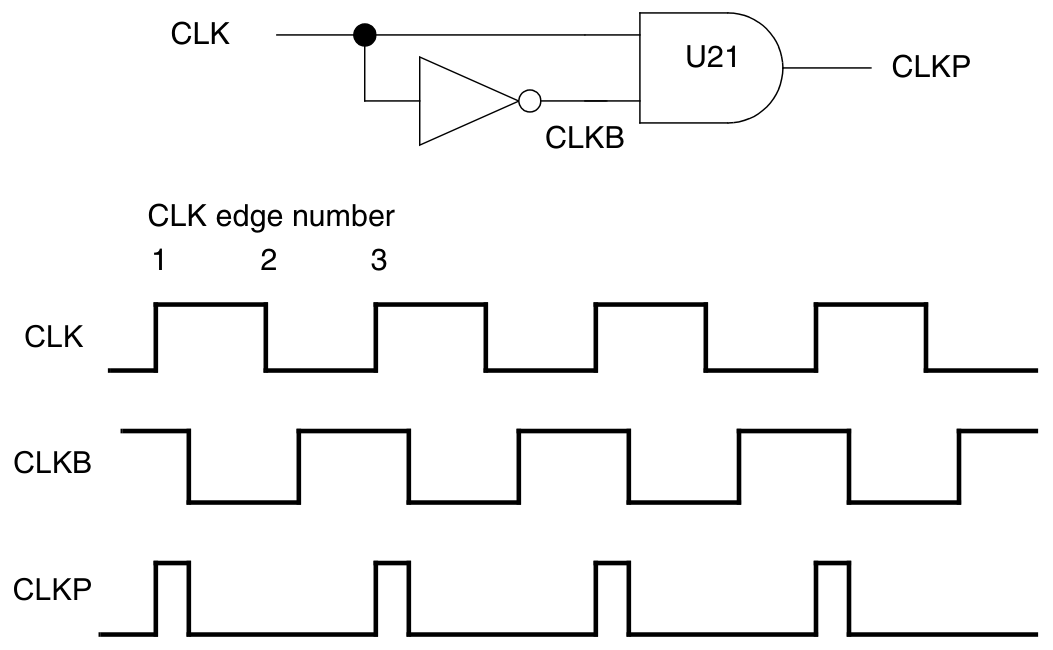
\includegraphics[width=0.78\textwidth]{fig-2-11.png}
  \caption{指定为生成时钟的脉冲时钟}
  \label{fig:pulse}
\end{figure}

把生成脉冲时钟 \cmd{CLKP} 指定为生成时钟：
\begin{lstlisting}
icc2_shell> create_generated_clock -name CLKP -source CLK \
    -edges {1 1 3} [get_pins U21/z]
\end{lstlisting}

\subsection{用 set\_sense 定义脉冲时钟}
\subsubsection*{Defining a Pulse Clock With the set\_sense Command}

可以用 \cmd{set\_sense} 的 \opt{-pulse} 把已有时钟指定为脉冲时钟：
\begin{itemize}
  \item 上升沿触发的高脉冲：\opt{-pulse rise\_triggered\_high\_pulse}。
  \item 上升沿触发的低脉冲：\opt{-pulse rise\_triggered\_low\_pulse}。
  \item 下降沿触发的高脉冲：\opt{-pulse fall\_triggered\_high\_pulse}。
  \item 下降沿触发的低脉冲：\opt{-pulse fall\_triggered\_low\_pulse}。
\end{itemize}

脉冲时钟不定义为单独的时钟域。只是源时钟的指定极性从时钟网络中该点向下游传播。

下列命令指定单元 \cmd{U21} 输出上的时钟是一个在源时钟上升沿既上升又下降的脉冲：
\begin{lstlisting}
prompt> set_sense -pulse rise_triggered_high_pulse \
    [get_pins U21/z]
\end{lstlisting}

\subsection{指定脉冲时钟的标称宽度}
\subsubsection*{Specifying the Nominal Width of a Pulse Clock}

无论使用库中定义的脉冲发生器单元、\cmd{create\_generated\_clock} 还是 \cmd{set\_sense}，所产生脉冲的标称宽度都是零。要得到实际脉冲宽度，工具考虑脉冲发生器输出引脚上上升与下降 latency 的差异：
\begin{quote}
（高脉冲宽度）=（下降 network latency）$-$（上升 network latency）\\
（低脉冲宽度）=（上升 network latency）$-$（下降 network latency）
\end{quote}

可以用 \cmd{set\_clock\_latency} 为理想时钟显式指定 latency（从而指定脉冲宽度），也可以让工具为传播时钟从电路计算传播 latency。

例如，要把单元 \cmd{U21} 输出下游全部寄存器的高脉冲理想宽度设为 0.5，且总 latency 为 0.6：
\begin{lstlisting}
icc2_shell> set_clock_latency -rise 0.6 [get_pins and2.z]
icc2_shell> set_clock_latency -fall 1.1 [get_pins and2.z]
\end{lstlisting}

\section{设置并报告最小脉冲宽度约束}
\subsection*{Setting and Reporting Minimum Pulse Width Constraints}

由于上升沿与下降沿传播延迟不同，寄存器处的时钟脉冲宽度可能变窄。若寄存器时钟引脚上的脉冲过窄，寄存器可能无法正确采集数据。因此，满足最小脉冲宽度约束是时序电路正确工作所必需的。

库单元引脚可以定义最小脉冲宽度。此外，可以用 \cmd{set\_min\_pulse\_width} 为指定时钟或时钟引脚显式设置脉冲宽度约束。

默认同时约束时钟的高脉冲与低脉冲。若只约束高脉冲或低脉冲，使用 \opt{-high} 或 \opt{-low}。

下例把 \cmd{reg1/CK} 上时钟信号的高、低最小脉冲宽度分别设为 0.6 与 1.0：
\begin{lstlisting}
set_min_pulse_width -high 0.6 reg1/CK
set_min_pulse_width -low 1.0 reg1/CK
\end{lstlisting}

用 \cmd{report\_min\_pulse\_width} 或 \cmd{report\_constraints -min\_pulse\_width} 检查脉冲宽度违例。
\begin{lstlisting}
icc2_shell> report_min_pulse_width
...
                    Required      Actual
  Pin               pulse width   pulse width   Slack
  -----------------------------------------------------
 reg1/CK(low)        1.00          0.87         -0.13
 reg1/CK(high)       0.60          1.13          0.53
\end{lstlisting}

用 \cmd{remove\_min\_pulse\_width} 去掉这些约束。

\section{定义时钟组之间的关系}
\subsection*{Defining the Relationship Between Clock Groups}

对多时钟设计，时序分析默认检查所有时钟之间的时序路径。若某些时钟之间没有交互，可用 \cmd{set\_clock\_groups} 说明这一点，从而缩短时序分析的运行时间。

使用 \cmd{set\_clock\_groups} 时必须指定：
\begin{itemize}
  \item 时钟组之间的关系，为下列之一：
  \begin{itemize}
    \item \opt{-physically\_exclusive}：物理互斥。工具假定这些时钟组在设计中不同时存在，因此不检查它们之间的时序路径，也不在这些时钟组的网线之间做串扰分析。
    \item \opt{-logically\_exclusive}：逻辑互斥。工具假定这些时钟组之间没有相位关系，因此不检查时钟之间的时序路径，但仍在这些时钟组的网线之间做串扰分析。
    \item \opt{-asynchronous}：异步。工具假定这些时钟组之间没有相位关系，因此不检查时钟之间的时序路径，但仍用无限到达时间窗口在这些时钟组的网线之间做串扰分析。
  \end{itemize}
  \item 用 \opt{-group} 一次或多次指定一个或多个时钟组。
  \begin{itemize}
    \item 只指定一次时，工具假定该组中的时钟与设计中所有其他时钟之间具有所指定的关系。
    \item 指定两次或更多次时，工具假定每一对时钟组之间具有所指定的关系。
  \end{itemize}
\end{itemize}

还可以：
\begin{itemize}
  \item 用 \opt{-name} 为时钟分组命名。若不命名，工具为每个分组推导一个唯一名称。
  \item 对用 \opt{-asynchronous} 指定的异步分组，用 \opt{-allow\_paths} 允许指定时钟之间仍做时序分析。
\end{itemize}

用 \cmd{remove\_clock\_groups} 去掉由 \cmd{set\_clock\_groups} 声明的时钟分组。

例如，指定时钟 \cmd{CK1} 相对设计中所有其他时钟物理互斥：
\begin{lstlisting}
icc2_shell> set_clock_groups -physically_exclusive -group {CK1}
\end{lstlisting}

指定时钟 \cmd{CK2}、\cmd{CK3} 与时钟 \cmd{CK4}、\cmd{CK5} 逻辑互斥：
\begin{lstlisting}
icc2_shell> set_clock_groups -logically_exclusive \
    -group {CK2 CK3} -group {CK4 CK5}
\end{lstlisting}

指定时钟 \cmd{CK6}、\cmd{CK7} 与 \cmd{CK8} 彼此异步：
\begin{lstlisting}
icc2_shell> set_clock_groups -asynchronous \
    -group {CK6} -group {CK7} -group {CK8}
\end{lstlisting}

\section{报告时钟相关信息}
\subsection*{Reporting Clock Related Information}

用 \cmd{report\_clocks} 报告由 \cmd{create\_clock} 与 \cmd{create\_generated\_clock} 定义的时钟。默认报告：
\begin{itemize}
  \item 全部时钟的周期、波形、属性与源。
  \item 全部生成时钟的 master 时钟源、master 时钟名以及波形修改方式。
\end{itemize}

还可以报告：
\begin{itemize}
  \item 通过指定时钟名，只报告所选时钟。
  \item 用 \opt{-skew} 报告理想时钟网络特性，包括用 \cmd{set\_clock\_latency} 指定的 source 与 network latency、用 \cmd{set\_clock\_uncertainty} 指定的不确定性，以及用 \cmd{set\_clock\_transition} 指定的理想转换时间。
  \item 用 \opt{-groups} 报告由 \cmd{set\_clock\_groups} 指定的时钟分组。
  \item 用 \opt{-modes} 报告所选 mode 的时钟信息。
\end{itemize}

用 \cmd{get\_clocks} 或 \cmd{all\_clocks} 创建时钟 collection。时钟对象与同名端口对象要用 \cmd{get\_clocks} 与 \cmd{get\_ports} 区分。

例如，报告周期小于或等于 15.0 的时钟：
\begin{lstlisting}
icc2_shell> report_clocks [get_clocks -filter "period <= 15.0" *]
...
Attributes:
    d - dont_touch_network
    f - fix_hold
    p - propagated_clock
    G - generated_clock
Clock          Period   Waveform            Attrs     Sources
------------------------------------------------------------------------
PCI_CLK         15.00   {0 7.5}                       {pclk}
SDRAM_CLK        7.50   {0 3.75}                      {sdram_clk}
SD_DDR_CLK       7.50   {0 3.75}            G         {sd_CK}
SYS_CLK          8.00   {0 4}                         {sys_clk}
------------------------------------------------------------------------
Generated     Master         Generated      Master         Waveform
Clock         Source         Source         Clock          Modification
------------------------------------------------------------------------
SD_DDR_CLK    sdram_clk      {sd_CK}        SDRAM_CLK      divide_by(1)
------------------------------------------------------------------------
\end{lstlisting}

\section{删除时钟}
\subsection*{Removing Clocks}

\begin{itemize}
  \item 用 \cmd{remove\_clocks} 删除由 \cmd{create\_clock} 创建的真实时钟或虚拟时钟。
  \item 用 \cmd{remove\_generated\_clocks} 删除由 \cmd{create\_generated\_clock} 创建的生成时钟。
\end{itemize}
